% Captions for the two primary RPS23 figures. Requires graphicx.
\begin{figure}[t]
\centering
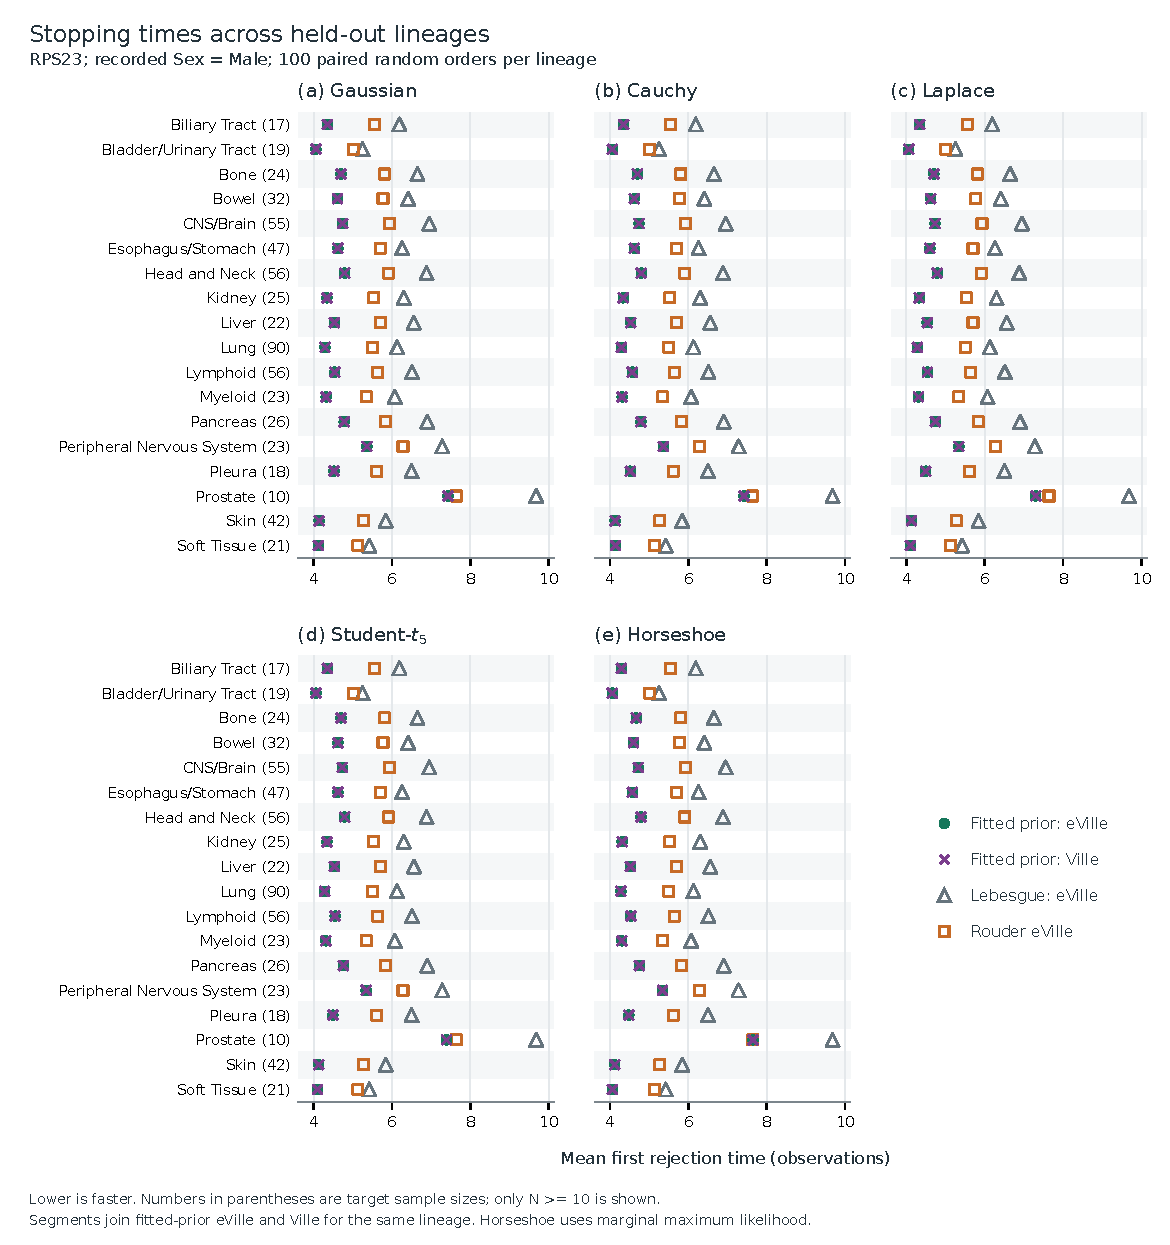
\includegraphics[width=\textwidth]{results/figures/raw_stopping_times_all_lineages.pdf}
\caption{Mean first rejection times for RPS23 in male cell lines, using 100
paired random observation orders in each of 18 held-out lineages. Each panel
corresponds to a source-fitted prior. Segments join fitted-prior eVille and
Ville means; Lebesgue and Rouder eVille benchmarks use the same target and
orders. Numbers in parentheses are target sample sizes. All lineages have
at least ten observations, and all procedures reject in every evaluated
random order. Horseshoe parameters use source-only constrained marginal
maximum likelihood.}
\label{fig:rps23-stopping}
\end{figure}

\begin{figure}[t]
\centering
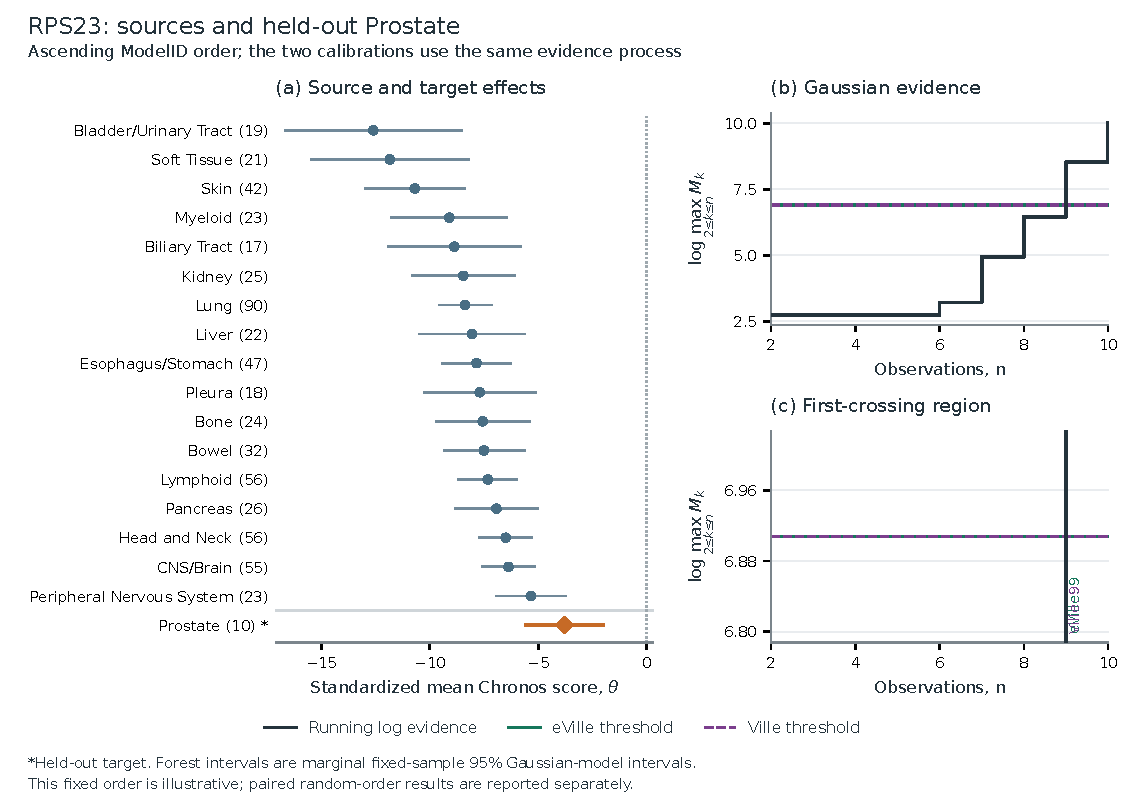
\includegraphics[width=\textwidth]{results/figures/example_forest_and_evidence.pdf}
\caption{Illustrative RPS23 analysis with Prostate held out.
(a) Source and target standardized mean Chronos scores, with marginal
fixed-sample 95\% intervals obtained by noncentral-$t$ inversion under the
Gaussian working model. (b) Running maximum of the Gaussian-prior
log-evidence in ascending ModelID order. (c) Enlargement of the crossing
region: eVille rejects at $n=2$ and Ville at $n=6$. The two calibrations use
the same evidence process. These fixed-order crossings are illustrative;
the corresponding means across 100 paired random orders are 3.51 and 3.94.
The gene and illustrative target were selected retrospectively.}
\label{fig:rps23-example}
\end{figure}
